\label{chap:transformer_forecaster}

\section{System Overview and Architectural Philosophy}
Continuous forecasting of postprandial glycemic excursions requires an architecture capable of processing two fundamentally disparate data types:
\begin{enumerate}
    \item \textbf{Dynamic Continuous Streams ($\mathbf{X}_{\text{seq}} \in \mathbb{R}^{60 \times 3}$):} A 60-minute historical sequence recorded at 1-minute intervals. It tracks continuous glucose levels, heart rate, and metabolic equivalents (METs) right before a meal to capture the person's current physiological state.
    \item \textbf{High-Dimensional Static Covariates ($\mathbf{x}_{\text{stat}} \in \mathbb{R}^{61}$):} Fixed features for each meal event, including nutritional values (carbs, protein, fat, fiber, calories), standard clinical lab tests, patient body metrics, and the 8 latent values extracted by our gut microbiome $\beta$-VAE.
\end{enumerate}

To synthesize these heterogeneous modalities without suffering from the spike dampening and baseline drift common in recurrent networks, we introduce \textbf{TransformerForecaster}. Figure \ref{fig:methodology_flowchart} provides an end-to-end architectural schematic of the pipeline, from raw telemetry ingestion to continuous postprandial trajectory prediction.

\begin{figure*}[!t]
\centering
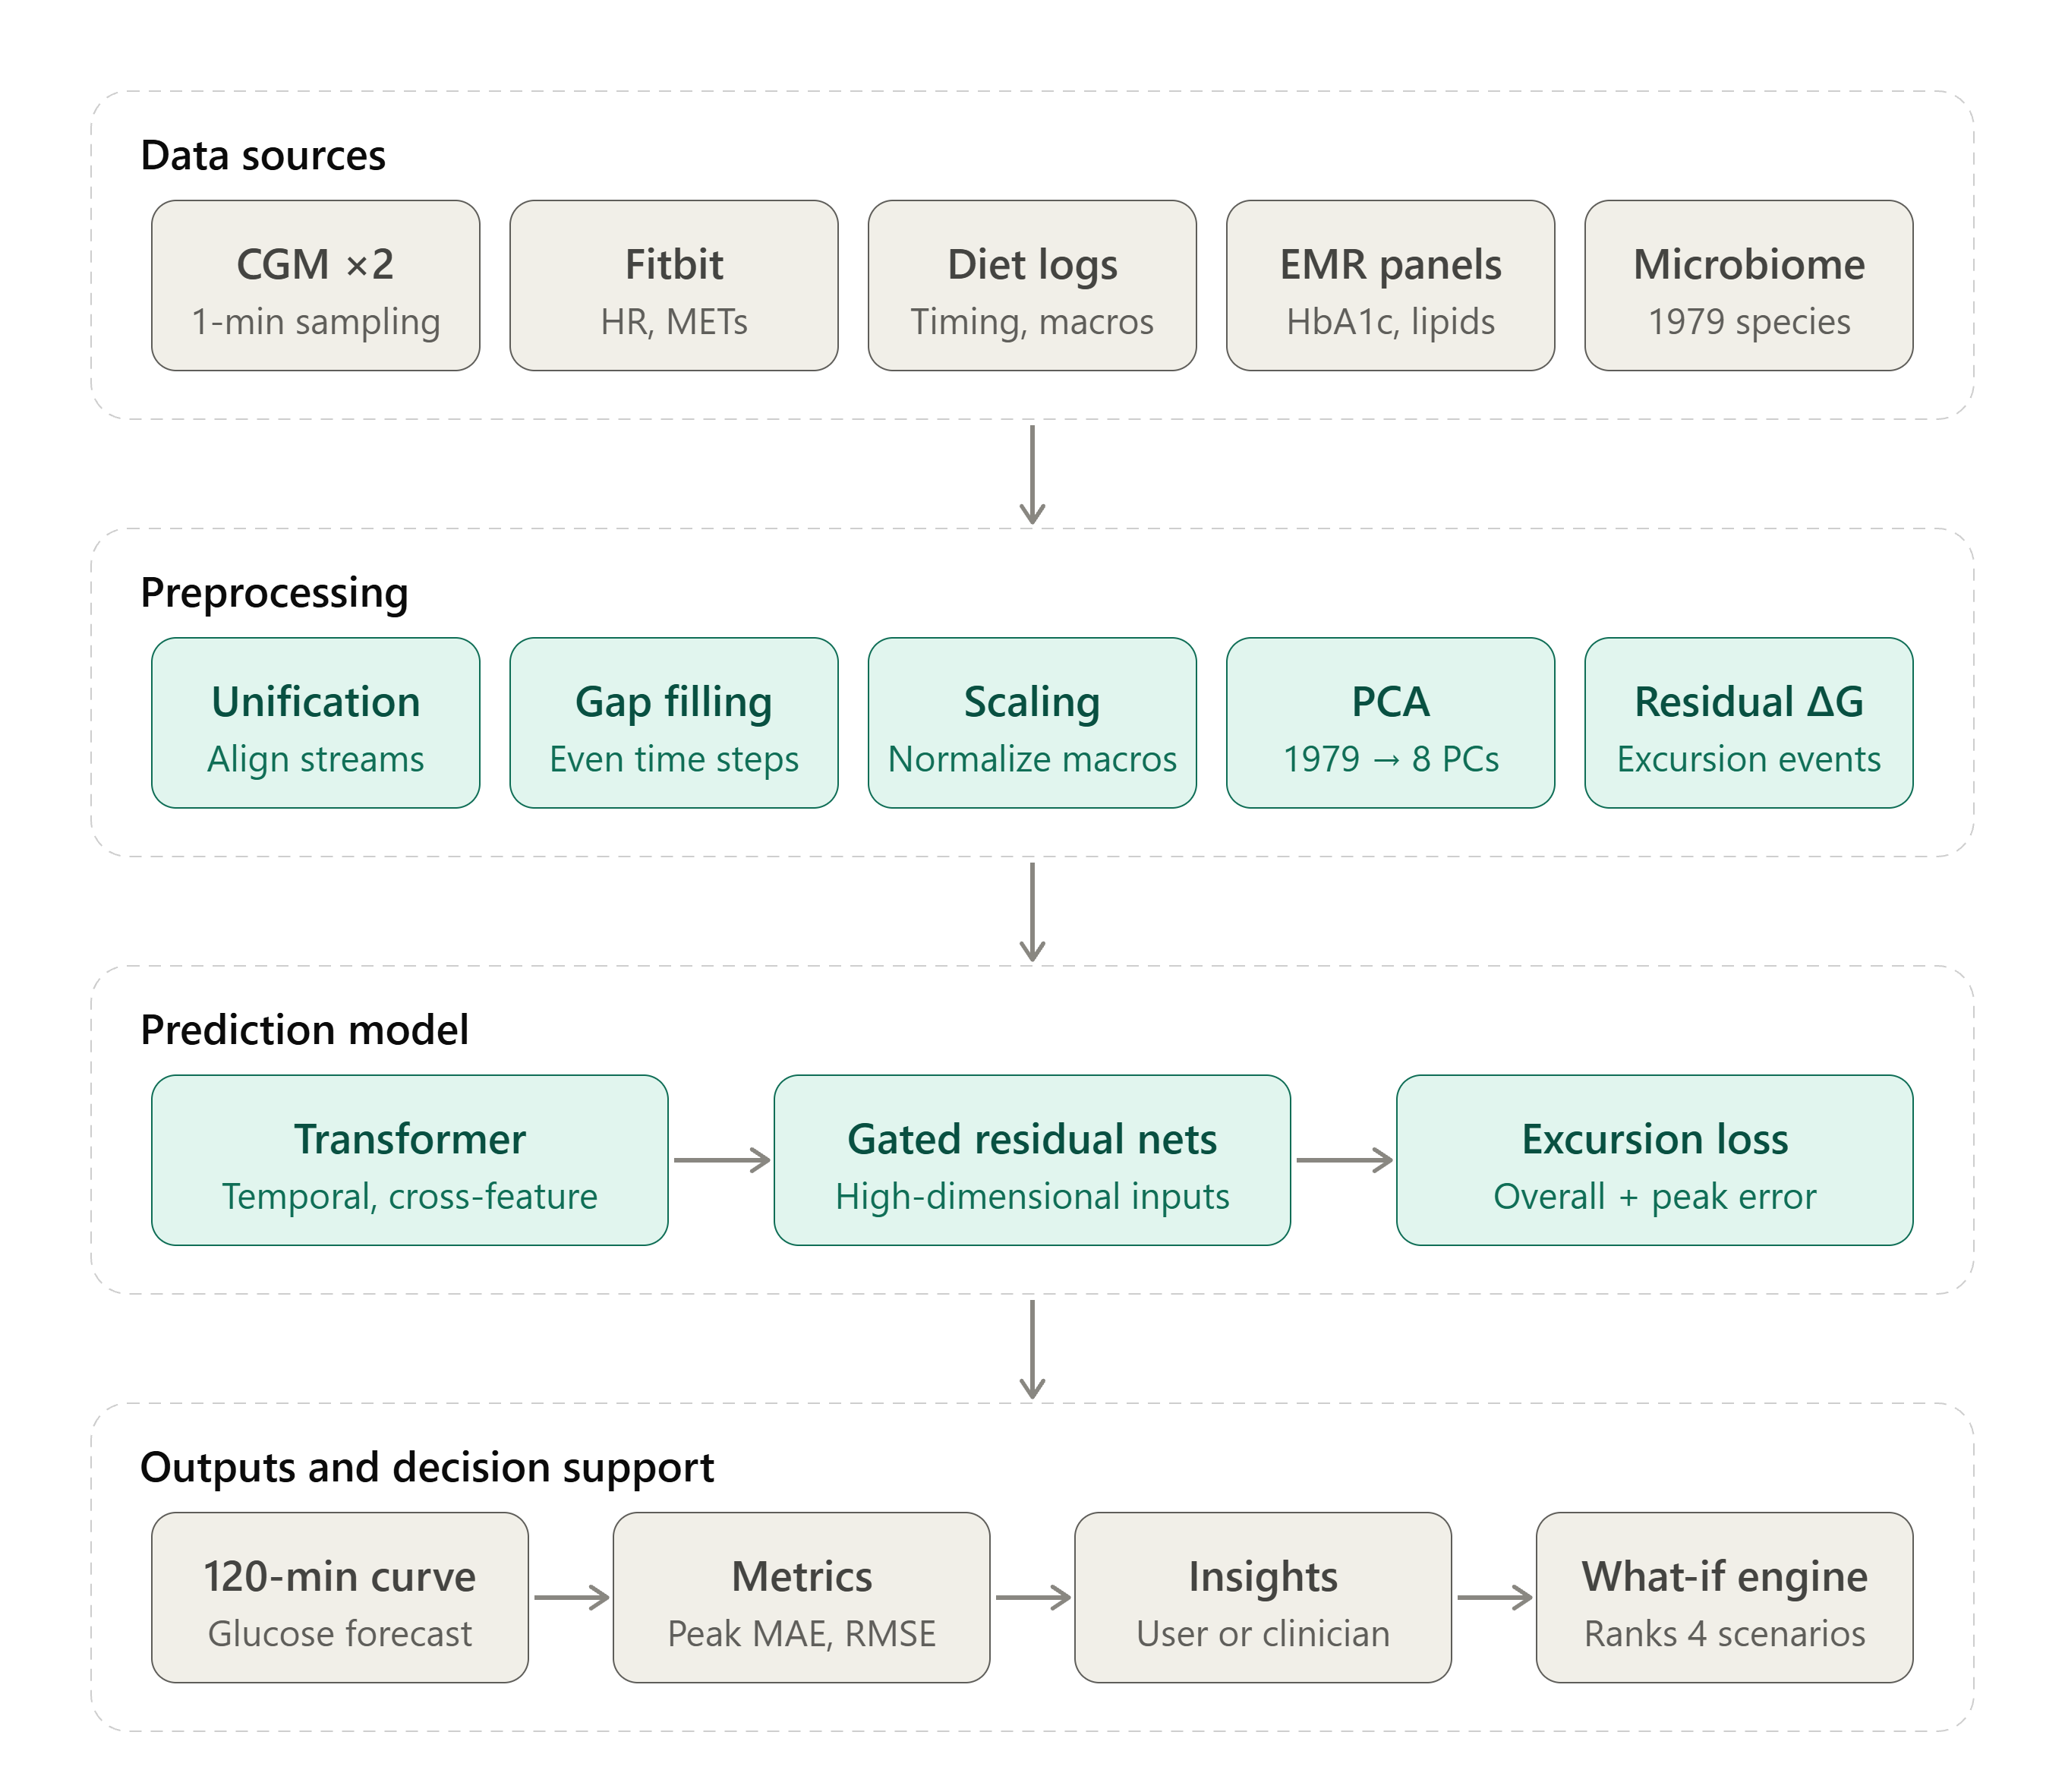
\includegraphics[width=0.95\textwidth]{images/t2d_digital_twin_architecture.png}
\caption{End-to-end system architecture of the GlycoTwin framework, detailing multi-modal data ingestion, Microbiome $\beta$-VAE latent extraction, TransformerForecaster neural architecture, and Causal What-If Simulation Engine.}
\label{fig:methodology_flowchart}
\end{figure*}

\section{Dynamic Pre-Meal Temporal Attention Encoder}
The 60-minute pre-meal telemetry sequence $\mathbf{X}_{\text{seq}} = [\mathbf{x}_1, \mathbf{x}_2, \dots, \mathbf{x}_{60}]^T \in \mathbb{R}^{60 \times 3}$ contains:
\begin{equation}
    \mathbf{x}_t = \big[ G(t), \text{HeartRate}(t), \text{METs}(t) \big]^T
\end{equation}

\subsection{Input Projection and Positional Encoding}
The dynamic vectors are projected into a $d_{\text{model}} = 64$ dimensional embedding space via a learnable linear transformation $\mathbf{W}_{\text{proj}} \in \mathbb{R}^{3 \times 64}$. To preserve temporal sequence order within the self-attention mechanism, we inject deterministic sinusoidal positional encodings \cite{vaswani2017attention}:
\begin{align}
    \mathbf{E}_0 &= \mathbf{X}_{\text{seq}} \mathbf{W}_{\text{proj}} + \mathbf{PE} \in \mathbb{R}^{60 \times 64} \\
    \mathbf{PE}_{(t, 2i)} &= \sin\left(\frac{t}{10000^{2i/d_{\text{model}}}}\right) \\
    \mathbf{PE}_{(t, 2i+1)} &= \cos\left(\frac{t}{10000^{2i/d_{\text{model}}}}\right)
\end{align}
for temporal step $t \in \{1, \dots, 60\}$ and channel index $i \in \{0, \dots, 31\}$.

\subsection{Multi-Head Self-Attention (MHSA) Layers}
We pass the embedded input through $L = 2$ Transformer Encoder layers. Each layer uses a Multi-Head Self-Attention (MHSA) block with $h = 4$ parallel heads (giving head dimension $d_k = d_{\text{model}} / h = 16$). After attention, the features pass through a feed-forward network (FFN) with Gaussian Error Linear Unit (GELU) non-linearity and a hidden dimension of $d_{\text{ff}} = 128$:
\begin{align}
    \mathbf{Q}_i &= \mathbf{E}_{l-1} \mathbf{W}_i^Q, \quad \mathbf{K}_i = \mathbf{E}_{l-1} \mathbf{W}_i^K, \quad \mathbf{V}_i = \mathbf{E}_{l-1} \mathbf{W}_i^V \\
    \text{head}_i &= \text{softmax}\left(\frac{\mathbf{Q}_i \mathbf{K}_i^T}{\sqrt{d_k}}\right) \mathbf{V}_i \\
    \mathbf{E}_l' &= \text{LayerNorm}\Big(\mathbf{E}_{l-1} + \text{Dropout}\big([\text{head}_1, \dots, \text{head}_h]\mathbf{W}^O\big)\Big) \\
    \mathbf{E}_l &= \text{LayerNorm}\Big(\mathbf{E}_l' + \text{Dropout}\big(\text{GELU}(\mathbf{E}_l' \mathbf{W}_1^{\text{ff}} + \mathbf{b}_1^{\text{ff}})\mathbf{W}_2^{\text{ff}} + \mathbf{b}_2^{\text{ff}}\big)\Big)
\end{align}

\subsection{Temporal Context Pooling}
To summarize the 60 time steps into a single vector representing the pre-meal state, we apply average pooling across the temporal dimension:
\begin{equation}
    \mathbf{h}_{\text{temp}} = \frac{1}{60} \sum_{t=1}^{60} \mathbf{E}_{L, t} \in \mathbb{R}^{64}
\end{equation}
This pooled vector $\mathbf{h}_{\text{temp}}$ holds summary information about pre-meal glucose trends, recent physical activity, and heart rate patterns.

\section{Gated Residual Network (GRN) for Static Modalities}
The static input vector $\mathbf{x}_{\text{stat}} \in \mathbb{R}^{61}$ includes meal nutritional values, clinical lab tests, patient body metrics, and the 8-dimensional gut microbiome latent features ($\mathbf{z}_{\text{microbiome}}$). 

If we simply concatenate these 61 static variables directly into the neural network, less informative or noisy features can hurt the model's performance. To handle this, we process static covariates with a \textbf{Gated Residual Network (GRN)} \cite{lim2021temporal}. The GRN learns non-linear combinations of features while using a gating mechanism to suppress irrelevant signals and let key predictors (like meal carbohydrates or insulin resistance markers) pass through:
\begin{align}
    \mathbf{\eta}_1 &= \text{ELU}(\mathbf{W}_1 \mathbf{x}_{\text{stat}} + \mathbf{b}_1) \in \mathbb{R}^{64} \\
    \mathbf{\eta}_2 &= \text{Dropout}\big(\mathbf{W}_2 \mathbf{\eta}_1 + \mathbf{b}_2, p=0.1\big) \in \mathbb{R}^{64} \\
    \mathbf{g} &= \sigma(\mathbf{W}_g \mathbf{\eta}_2 + \mathbf{b}_g) \in \mathbb{R}^{64} \quad \text{(Gating Mechanism)} \\
    \mathbf{h}_{\text{stat}} &= \text{LayerNorm}\Big(\mathbf{W}_{\text{skip}} \mathbf{x}_{\text{stat}} + \mathbf{g} \odot \mathbf{\eta}_2\Big) \in \mathbb{R}^{64}
\end{align}
Here, $\text{ELU}(x) = \max(0, x) + \min(0, \exp(x) - 1)$ provides smooth gradients for negative values, $\sigma(\cdot)$ is the sigmoid gating function, and $\mathbf{W}_{\text{skip}} \in \mathbb{R}^{64 \times 61}$ provides a linear skip connection to retain direct linear relationships.

\section{Multi-Modal Fusion and Projection Decoder}
The dynamic temporal representation $\mathbf{h}_{\text{temp}} \in \mathbb{R}^{64}$ and the gated static representation $\mathbf{h}_{\text{stat}} \in \mathbb{R}^{64}$ are concatenated into a fused multi-modal embedding:
\begin{equation}
    \mathbf{h}_{\text{fused}} = [\mathbf{h}_{\text{temp}} \,\|\, \mathbf{h}_{\text{stat}}] \in \mathbb{R}^{128}
\end{equation}

The fused representation feeds a multi-layer projection decoder composed of dense layers, LeakyReLU activations, Dropout ($p=0.15$), and Layer Normalization, projecting directly to the $H = 24$ multi-horizon forecasting steps:
\begin{align}
    \mathbf{h}_{\text{dec}, 1} &= \text{LeakyReLU}\Big(\text{LayerNorm}\big(\mathbf{W}_{d1} \mathbf{h}_{\text{fused}} + \mathbf{b}_{d1}\big)\Big) \in \mathbb{R}^{128} \\
    \mathbf{h}_{\text{dec}, 2} &= \text{LeakyReLU}\Big(\text{LayerNorm}\big(\mathbf{W}_{d2} \mathbf{h}_{\text{dec}, 1} + \mathbf{b}_{d2}\big)\Big) \in \mathbb{R}^{64} \\
    \hat{\boldsymbol{\Delta \mathbf{G}}} &= \mathbf{W}_{\text{out}} \mathbf{h}_{\text{dec}, 2} + \mathbf{b}_{\text{out}} \in \mathbb{R}^{24}
\end{align}

\section{Residual Delta Trajectory Formulation ($\Delta G_t = G_t - G_0$)}
One major difficulty when predicting post-meal blood glucose directly is \textbf{baseline offset bias}. Different patients start meals at very different starting glucose levels—ranging from roughly $85\text{ mg/dL}$ in healthy subjects to over $160\text{ mg/dL}$ in uncontrolled type 2 diabetes. When a model tries to predict raw absolute values $\hat{G}(t)$ directly across all patients, standard loss functions often cause it to predict values close to the overall dataset average ($\approx 120\text{ mg/dL}$). This leads to over-predicting healthy participants, under-predicting diabetic participants, and flattening out the post-meal peaks.

To avoid this problem, we train the model to predict the \textbf{relative post-meal glucose rise}:
\begin{equation}
    \Delta G(t) = G(t) - G_0, \quad \forall t \in \{5, 10, 15, \dots, 120\text{ min}\}
\end{equation}
where $G_0 = G(t_{\text{meal}})$ is the glucose reading at the exact start of the meal.

During testing and evaluation, we reconstruct the final predicted glucose curve by adding this change back to the baseline:
\begin{equation}
    \hat{G}(t) = G_0 + \max\Big(0, \hat{\Delta G}(t)\Big)
\end{equation}
We include the non-negative threshold $\max(0, \cdot)$ because eating carbohydrates causes glucose to rise rather than drop below the pre-meal baseline during the initial postprandial period.

\section{Multi-Objective Composite Excursion Loss Function}
Standard Mean Squared Error (MSE) measures point-by-point errors equally:
\begin{equation}
    \mathcal{L}_{\text{MSE}} = \frac{1}{H} \sum_{k=1}^{H} \big(\hat{Y}_k - Y_k\big)^2
\end{equation}
In practice, a model trained only on MSE can get an acceptable score simply by predicting a flat line through the middle of the actual curve. However, this misses the highest glucose spike, which is the most critical information for diabetes management.

From a medical perspective, two factors are essential during a post-meal response:
\begin{enumerate}
    \item \textbf{Peak Excursion Magnitude ($G_{\max}$):} The highest glucose level reached after the meal.
    \item \textbf{Glycemic Rate-of-Change ($\nabla G$):} How quickly glucose rises and recovers over time.
\end{enumerate}

To make sure our model captures these aspects, we trained it using a \textbf{Composite Excursion Loss Function}:
\begin{equation}
    \mathcal{L}_{\text{total}} = \mathcal{L}_{\text{MSE}}(\hat{\mathbf{Y}}, \mathbf{Y}) + \lambda_1 \mathcal{L}_{\text{peak}}(\hat{\mathbf{Y}}, \mathbf{Y}) + \lambda_2 \mathcal{L}_{\text{deriv}}(\hat{\mathbf{Y}}, \mathbf{Y})
\end{equation}
where:
\begin{align}
    \mathcal{L}_{\text{peak}} &= \Big| \max_{k}(\hat{Y}_k) - \max_{k}(Y_k) \Big| \\
    \mathcal{L}_{\text{deriv}} &= \frac{1}{H-1} \sum_{k=1}^{H-1} \Big| (\hat{Y}_{k+1} - \hat{Y}_k) - (Y_{k+1} - Y_k) \Big|^2
\end{align}
We set the hyperparameter weights to $\lambda_1 = 0.6$ for the peak error and $\lambda_2 = 0.3$ for the slope error. This combined loss encourages the model to accurately predict both the peak value and the overall shape of the curve.

\section{Optimization and Regularization Strategy}
TransformerForecaster was optimized end-to-end using the \textbf{AdamW optimizer} with decoupled weight decay ($1 \times 10^{-4}$). Training utilized a \textbf{Cosine Annealing Learning Rate Scheduler} with an initial learning rate $\eta_0 = 1 \times 10^{-3}$ decaying to $\eta_{\min} = 1 \times 10^{-5}$ across 120 epochs. Early stopping with a patience of 20 epochs based on validation loss prevented overfitting. Gradient norms were clipped to a maximum threshold of $1.0$ to ensure numerical stability during backpropagation.
